\chapter{Background}
\section{Software Artifacts}
\label{sec:sfs}

Software artifacts (or \sfs{}) come in a wide variety of forms and have existed 
since the first programs were created. In the broadest sense, we can think of 
\sfs{} as anything produced during the creation of a piece of software that 
serves some purpose. Any document detailing what the software should do, how it 
was designed, how it was implemented, how to test it, and so on would be 
considered a \sf{}, as would the source code whether as a text file, stack of 
punched cards, magnetic tapes, or other media.

\ds{Need to work in (here?) why \sfs{} are important}

\fig{
\begin{center}
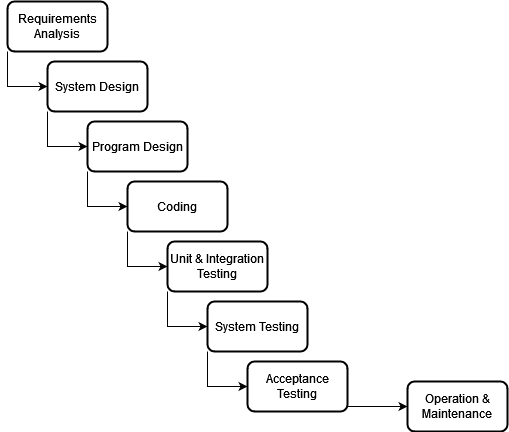
\includegraphics[width=\linewidth]{figures/Waterfall.png}
\end{center}}
{The Waterfall Model of Software Development}
{fig:Waterfall}

Software design can follow a number of different design processes, each with 
their own collection of \sfs{}. A common, traditional approach is the Waterfall 
model (Figure~\ref{fig:Waterfall}) of software 
development~\cite{PfleegerAndAtlee2010Ch2}. 
However, Parnas and Clements~\cite{ParnasAndClements1986} detailed what they 
dubbed a ``rational" design process; an idealized version of software 
development which includes what needs to be documented in corresponding \sfs{}.
The rational design process is not meant to be a linear process like the 
Waterfall model, but instead an iterative process using section stubs for 
information that is not yet available or not fully clear during the time of 
writing. Those stubs are then filled in over the development process, and 
existing documentation is updated so it appears to have been created in a 
linear fashion for ease of review later in the software lifecycle. The rational 
design process involves the following:

\begin{enumerate}
\item Establish/Document Requirements
\item Design and Document the Module Structure
\item Design and Document the Module Interfaces
\item Design and Document the Module Internal Structures
\item Write Programs
\item Maintain
\end{enumerate}

Parnas provided a list of the most important documents~\cite{Parnas2010} 
required for the rational design process, which Smith~\cite{Smith2016} 
\ds{which paper was it?} expanded upon by including complimentary artifacts 
such as source code, verification and validation plans, test cases, and build 
instructions. While there have been many proposed artifacts, the following 
curated list covers those most relevant to this thesis:

\begin{enumerate}
\item System Requirements
\item System Design Document
\item Module Guide
\item Module Interface Specification
\item Program Source Code
\item Verification and Validation Plan
\item Test cases
\item Verification and Validation Report
\item User Manual
\end{enumerate}

This list is not exhaustive of all the types of \sfs{}, as there are many other
design processes which use different types of \sfs{}. Looking at an agile 
approach using Scrum/Kanban, the \sfs{} tend to be distributed in different 
ways. Requirements are documented in tickets under so-called `epics', 
`stories', and `tasks' as opposed to a singular requirements artifact, and the 
acceptance criteria listed on those tickets make up the validation and 
verification plan. 

Regardless of the process used, most attempt to document very similar 
information to that of the rational design process. Using the waterfall model 
as an example, we can see (Table~\ref{tab:RatWatComp}) the rational design 
process and its artifacts map onto the model in a very straightforward manner.

\begin{table}[htbp]
\caption{Comparison of Rational Design Process and Waterfall Model}
\label{tab:RatWatComp}
\begin{tabular}{|p{.25\linewidth}|p{.35\linewidth}|p{.4\linewidth}|}
\hline &&\\
Rational Design phase & Corresponding Waterfall phase(s) & Common \SFS{}
\\&&\\ \hline &&\\
	Establish/ Document Requirements & Requirements Analysis & System 
	Requirements Specification \newline \newline
	Verification and Validation plan
\\&&\\ \hline &&\\
	Design and Document the Module Structure & 
	System Design  & 
	Design Document
\\&&\\ \hline &&\\
	Design and Document the Module Interfaces & 
	Program Design & 
	Module Interface Specification
\\&&\\ \hline &&\\
	Design and Document the Module Internal Structures &
	Program Design &
	Module Guide
\\&&\\ \hline &&\\
	Write Programs & 
	Coding &
	Source code  \newline \newline
	Build instructions
\\&&\\ \hline &&\\
	Maintain & 
	Unit \& Integration Testing \newline \newline System Testing \newline 
	\newline Acceptance 
	Testing \newline \newline Operation \& Maintenance &
	Test cases \newline \newline
	Verification and Validation Report
\\ \hline
\end{tabular}
\end{table}

\SFS{} are important to development in a number of ways, such as easing the 
burden of maintenance and training. We outline the artifacts we are most 
interested below with a brief description of their purpose.

\cardifact{Software Requirements Specification}{Contains the functional and 
nonfunctional requirements detailing what the desired software system should 
do.}
\cardifact{System Design Document}{Explains how the system should be broken 
down and documents implementation-level decisions that have been made for the 
design of the system.}
\cardifact{Module Guide}{In-depth explanation of the modules outlined in the 
System Design Document.}
\cardifact{Module Interface Specification}{Interface specification for each of 
the modules outlined in the System Design Document/Module Guide.}
\cardifact{Program Source Code}{The source code of the implemented software 
system.}
\cardifact{Verification and Validation Plan}{Uses the system requirements to 
document acceptance criteria for each requirement that can be validated.}
\cardifact{Test cases}{Implementation of the Verification and Validation Plan 
in source code (where applicable) or as a step-by-step guide for testers.}
\cardifact{Verification and Validation Report}{Report outlining the results 
after undertaking all of the testing initiatives outlined in the Verification 
and Validation plan and test cases.}

Parnas~\citep{Parnas2010} does an excellent job of defining the target audience 
for each of the most common \sfs{} and we extend that alongside our work. A 
summary can be found in Table~\ref{tab:sfsummary}.

\begin{table}[h]
\caption{A summary of the Audience for each of the most common \sfs{} and what 
problem that \sf{} is solving}
\label{tab:sfsummary}
\begin{tabular}{| P{.3\linewidth} | p{.3\linewidth}  | p{.3\linewidth} |}
\hline
 \SF{} & Who (Audience) & What (Problem)
\\ \hline
	SRS & 

	Software Architects \newline \newline
	QA analysts & 

	Define exactly what specification the software system must adhere to. 
\\ \hline
	Module Guide & 

	All developers \newline \newline
	QA analysts  & 

	Outline implementation decisions around the separation of functionality 
	into modules and give an overview of each module.
\\ \hline
	Module Interface Specifications & 

	Developers who implement the module \newline \newline
	Developers who use the module \newline \newline
	QA analysts & 

	Detail the exact interfaces of the modules from the Module Guide.
\\ \hline
	Verification and Validation Plan &
	
	Developers who implement the module \newline \newline
	QA analysts &

	Describe how the software should be verified using tests that can be 
	validated. Includes module-specific and system-wide plans.
\\ \hline
\end{tabular}
\end{table}

\section{Software Reuse and Software Families}
\subsection{Software/Program Families}
  - Bring up GNU/Linux and different distros as examples of software families
    - (Raspbian v Raspbian lite) = Debian--, etc.
\subsection{Reuse and Reproducible Research}
  - Touch on reuse areas like reproducible research - Gentleman and Lang 2012

Being able to reproduce results, is fundamental to the idea of good science.
When it comes to software projects, there are often many undocumented
assumptions or modifications (including hacks) involved in the finished product.
This can make replication impossible without the help of the original author,
and in some cases reveal errors in the original author's
work~\cite{IonescuAndJansson2013}.

Reproducible research has been used to mean embedding executable code in
research papers to allow readers to reproduce the results
described~\cite{SchulteEtAl2012}.

Combining research reports with relevant code, data, etc.\ is not necessarily
easy, especially when dealing with the publication versions of an author's work.
As such, the idea of \emph{compendia} were
introduced~\cite{GentlemanAndLang2012} to provide a means of encapsulating the
full scope of the work. Compendia allow readers to see computational details, as
well as re-run computations performed by the author. Gentleman and Lang proposed
that compendia should be used for peer review and distribution of scientific
work~\cite{GentlemanAndLang2012}.

Currently, several tools have been developed for reproducible research
including, but not limited to, Sweave~\cite{Leisch2002},
SASweave~\cite{LenthEtAl2007}, Statweave~\cite{Lenth2009},
Scribble~\cite{FlattEtAl2009}, and Org-mode~\cite{SchulteEtAl2012}. The most
popular of those being Sweave~\cite{SchulteEtAl2012}. The aforementioned tools
maintain a focus on code and certain computational details. Sweave,
specifically, allows for embedding code into a document which is run as the
document is being typeset so that up to date results are always included.
However, Sweave (along with many other tools), still maintains a focus on
producing a single, linear document. It is my hope that Drasil will outperform
these existing tools due to its flexibility and its ability to create multiple
artifacts from a knowledge base.

\section{Literate Approaches to Software Development}

There have been several approaches attempting to combine development of program 
code with documentation. Literate Programming and literate software are two 
such approaches that have influenced the direction of this thesis. Each of 
these approaches is outlined in the following sections.

\subsection{Literate Programming}

Literate Programming (LP) is a method for writing software introduced by Knuth 
that focuses on explaining to a human what we want a computer to do rather than 
simply writing a set of instructions for the computer on how to perform the 
task~\cite{Knuth1984}.

Developing literate programs involves breaking algorithms down into
\emph{chunks}~\cite{JohnsonAndJohnson1997} or \emph{sections}~\cite{Knuth1984}
which are small and easily understandable. The chunks are ordered to follow a 
``psychological order''~\cite{PieterseKourieAndBoake2004} if
you will, that promotes understanding. They do not have to be written in the 
same order that a computer would read them. It should also be noted that in a 
literate program, the code and documentation are kept together in one source. 
To extract runnable code, a process known as \emph{tangle} must be performed on 
the source. A similar process known as \emph{weave} is used to extract and 
typeset the documentation.

There are many advantages to LP beyond understandability. As a program is
developed and updated, the documentation surrounding the source code is more 
likely to be updated simultaneously. It has been experimentally found that 
using LP ends up with more consistent documentation and 
code~\cite{ShumAndCook1993}. There are many downsides to having inconsistent 
documentation while developing or maintaining 
code~\cite{Kotula2000,Thimbleby1986}, while the benefits of consistent 
documentation are numerous~\cite{Hyman1990, Kotula2000}. Keeping the advantages 
and disadvantages of good documentation in mind we can see that more effective, 
maintainable code can be produced if properly using 
LP~\cite{PieterseKourieAndBoake2004}.

Regardless of the benefits of LP, it has not been very popular with 
developers~\cite{ShumAndCook1993}. However, there are
several successful examples of LP's use in SC. Two such literate programs that 
come to mind are VNODE-LP~\cite{Nedialkov2006} and ``Physically Based 
Rendering: From Theory to Implementation''~\cite{PharrAndHumphreys2004} a 
literate program and textbook on the subject matter. Shum and 
Cook~\cite{ShumAndCook1993} discuss the main issues behind LP's lack of 
popularity which can be summed up as dependency on a 
particular output language or text processor, and the lack of flexibility on 
what should be presented or suppressed in the output.

There are several other factors which contribute to LP's lack of popularity and 
slow adoption thus far. While LP allows a developer to write their code and its 
documentation simultaneously, that documentation is comprised of a single 
artifact which may not cover the same material as standard artifacts software 
engineers expect (see Section~\ref{sec:sfs} for more details). LP also does not 
simplify the development process: documentation and code are written as usual, 
and there is the additional effort of re-ordering the chunks. The LP 
development process has some benefits such as allowing developers to follow a 
more natural flow in development by writing chunks in whichever order they 
wish, keep the documentation and code updated simultaneously (in theory) 
because of their co-location, and automatically incorporate code chunks into 
the documentation to reduce some information duplication.

There have been many attempts to increase LP's popularity by focusing on 
changing the output language or removing the text processor dependency. Several
new tools such as CWeb (for the C language), DOC++ (for C++), noweb 
(programming language independent), and others were developed. Other tools such 
as javadoc (for Java) and Doxygen (for multiple languages) were also influenced 
by LP, but differ in that they are merely document extraction tools. They do 
not contain the chunking features which allow for re-ordering algorithms.

With new tools came new features including, but not limited to, phantom
abstracting~\cite{ShumAndCook1993}, a ``What You See Is What You Get'' (WYSIWYG)
editor~\cite{FritzsonGunnarssonAndJirstrand2002}, and even movement away from 
the ``one source'' idea~\cite{Simonis2003}.

While LP is still not mainstream~\cite{Ramsey1994}, these more robust 
tools helped drive the understanding behind what exactly LP tools must 
do. In certain domains LP is becoming more standardized, for 
example: Agda, Haskell, and R support LP to some extent, even though it is not 
yet common practice. R has good tool support, with the most popular being
Sweave~\cite{Leisch2002}, however it is designed to dynamically create
up-to-date reports or manuals by running embedded code as opposed to being used
as part of the software development process. 

\subsection{Literate Software}

A combination of LP and Box Structure~\cite{Mills1986} was proposed as a new
method called ``Literate Software Development''
(LSD)~\cite{AlMatiiAndBoujarwah2002}. Box structure can be summarized as the
idea of different views which are abstractions that communicate the same
information in different levels of detail, for different purposes. Box
structures consist of black box, state machine, and clear box structures. The
black box gives an external (user) view of the system and consists of stimuli
and responses; the state machine makes the state data of the system visible (it
defines the data stored between stimuli); and the clear box gives an internal
(designer's) view describing how data are processed, typically referring to
smaller black boxes~\cite{Mills1986}. These three structures can be nested as
many times as necessary to describe a system.

LSD was developed with the intent to overcome the disadvantages of both LP and
box structure. It was intended to overcome LP's inability to specify interfaces
between modules, the inability to decompose boxes and implement the design
created by box structures, as well as the lack of tools to support box
structure~\cite{Deck1996}.

The framework developed for LSD, ``WebBox'', expanded LP and box structures in a
variety of ways. It included new chunk types, the ability to refine chunks, the
ability to specify interfaces and communication between boxes, and the ability
to decompose boxes at any level. However, literate software (and LSD) remains
primarily code-focused with very little support for creating other software
artifacts, in much the same way as LP.

\section{Generative Programming}
 - ?
